\documentclass[17pt]{extarticle}
\usepackage{amsmath, amssymb}
\usepackage{nccmath}
\usepackage[a4paper, total={6.5in, 10.5in},top=5mm,left=27mm]{geometry}
\usepackage{titlesec}
\usepackage{tikz}
\usepackage{gensymb}
\usetikzlibrary{arrows.meta}

\titleformat{\section}
{\normalfont\normalsize\bfseries}{\thesection}{1em}{}
\setcounter{secnumdepth}{0} %% no numbering for sections

\begin{document}
\noindent
\begin{fleqn} 

%%%%%%%%%%%%%%%%%%%%%%%%%%%%%%%%%%%%%%%%%%%%%%%%%%%%%%%%%%%%%%%%

\section{Question: 01}
Find the joint equation fo the pair of lines through the origin and making an equilateral triangle with the line $y = 3.$

%----------------------------------------

\section{Answer: 01}
Let OA and OB be the lines passing through the origin making an angle of
 $ 60\degree$ with the line $y = 3.$ \\
$\therefore$ OA and OB make an angle of $60\degree$ and $ 120\degree$ with the positive direction of X-axis. 
\begin{equation} \nonumber
\begin{alignedat}{4}
\text {Slope of line OA = tan}\ 60\degree = \sqrt{3} \\
\therefore \text {Equation of the line OA is}\\  
y= \sqrt{3}\ x \ i.e. \sqrt{3}\ x - y = 0 \\ 
\text {Slope of line OB = tan 120\degree} \\
\text {= tan (180 - 60)\degree} = \text{-tan}\ 60\degree\\
\therefore \text {Slope of line OB} = -\sqrt{3} \\
\therefore \text{Equation of the line OB is}\\  
\end{alignedat}
%\vrule
\quad\quad
\begin{alignedat}{4}
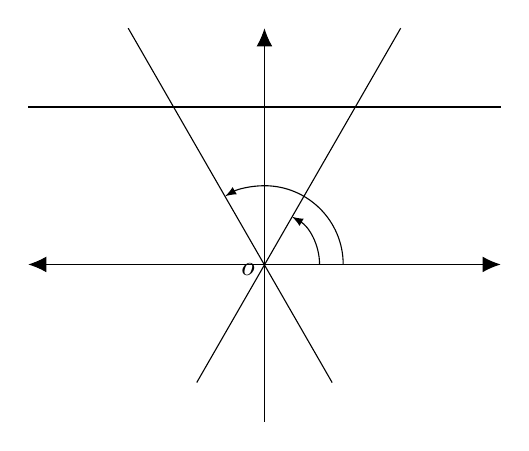
\begin{tikzpicture}
\draw [>={LaTeX[width=2mm,length=2.3mm]},<->](-3,0) -- (3,0);
\draw [>={LaTeX[width=2mm,length=2.3mm]},->](0,-2)  -- (0,3);
\draw (-3,2) -- (3,2);
\draw (-0.86,-1.5) -- (1.73,3);
\draw (-1.73,3) -- (0.86,-1.5);
\draw (0,0) node[anchor=north east,yshift=4pt] {$o$} ;
\draw[-latex] (0:0.7cm) arc (0:60:0.7cm);
\draw[-latex] (0:1cm) arc (0:120:1cm);
\end{tikzpicture}
\end{alignedat}
\end{equation}
\quad


\begin{equation} \nonumber
\begin{alignedat}{4}
y= -\sqrt{3}\ x \ i.e. \sqrt{3}\ x + y = 0 \\
\therefore \text {The joint equation the lines is}\\
\end{alignedat}
\quad
\vrule
\quad
\begin{alignedat}{4}
\left( \sqrt{3}\ x - y\right) \left( \sqrt{3}\ x + y\right) = 0 \\
i.e.\  3x^2 - y^2 = 0.
\end{alignedat}
\end{equation}

%%%%%%%%%%%%%%%%%%%%%%%%%%%%%%%%%%%%%%%%%%%%%%%%%%%%%%%%%%%%%%%%%%%%%%%%%%

\section{Question: 02}
Find the joint equation fo the pair of lines through the origin and making an equilateral triangle with the line $x = 3.$

%----------------------------------------

\section{Answer: 02}
Let OA and OB be the lines passing through the origin making an angle of
 $ 60\degree$ with the line $y = 3.$ \\
$\therefore$ OA and OB make an angle of $60\degree$ and $ 120\degree$ with the positive direction of X-axis. 
\begin{equation} \nonumber
\begin{alignedat}{4}
\text {Slope of line OA = tan}\ 60\degree = \sqrt{3} \\
\therefore \text {Equation of the line OA is}\\  
y= \sqrt{3}\ x \ i.e. \sqrt{3}\ x - y = 0 \\ 
\text {Slope of line OB = tan 120\degree} \\
\text {= tan (180 - 60)\degree} = \text{-tan}\ 60\degree\\
\therefore \text {Slope of line OB} = -\sqrt{3} \\
\therefore \text{Equation of the line OB is}\\  
\end{alignedat}
%\vrule
\quad\quad
\begin{alignedat}{4}
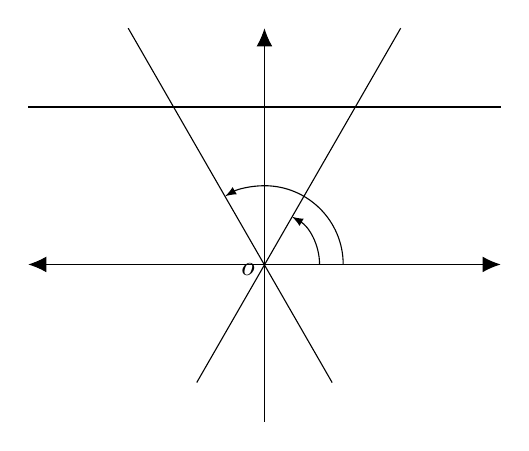
\begin{tikzpicture}
\draw [>={LaTeX[width=2mm,length=2.3mm]},<->](-3,0) -- (3,0);
\draw [>={LaTeX[width=2mm,length=2.3mm]},->](0,-2)  -- (0,3);
\draw (-3,2) -- (3,2);
\draw (-0.86,-1.5) -- (1.73,3);
\draw (-1.73,3) -- (0.86,-1.5);
\draw (0,0) node[anchor=north east,yshift=4pt] {$o$} ;
\draw[-latex] (0:0.7cm) arc (0:60:0.7cm);
\draw[-latex] (0:1cm) arc (0:120:1cm);
\end{tikzpicture}
\end{alignedat}
\end{equation}
\quad


\begin{equation} \nonumber
\begin{alignedat}{4}
y= -\sqrt{3}\ x \ i.e. \sqrt{3}\ x + y = 0 \\
\therefore \text {The joint equation the lines is}\\
\end{alignedat}
\quad
\vrule
\quad
\begin{alignedat}{4}
\left( \sqrt{3}\ x - y\right) \left( \sqrt{3}\ x + y\right) = 0 \\
i.e.\  3x^2 - y^2 = 0.
\end{alignedat}
\end{equation}

%%%%%%%%%%%%%%%%%%%%%%%%%%%%%%%%%%%%%%%%%%%%%%%%%%%%%%%%%%%%%%%%%%%%%%%%%%

\end{fleqn}
\end{document} 